\documentclass{article}%
\usepackage[T1]{fontenc}%
\usepackage[utf8]{inputenc}%
\usepackage{lmodern}%
\usepackage{textcomp}%
\usepackage{lastpage}%
\usepackage[head=40pt,margin=0.5in,bottom=0.6in]{geometry}%
\usepackage{graphicx}%
%
\title{\textbf{Lorent Saleh asegura que no está desterrado y volverá}}%
\author{Diario El Universal}%
\date{14/10/2018}%
%
\begin{document}%
\normalsize%
\maketitle%
\textbf{URL: }%
http://www.eluniversal.com/politica/23117/lorent{-}saleh{-}asegura{-}que{-}no{-}esta{-}desterrado{-}y{-}volvera\newline%
%
\textbf{Periodico: }%
EU, %
ID: %
23117, %
Seccion: %
politica\newline%
%
\textbf{Palabras Claves: }%
NO\_TIENE\newline%
%
\textbf{Derecho: }%
1.2%
, Otros Derechos: %
1.10%
, Sub Derechos: %
1.2.2, 1.10.1.1%
\newline%
%
\textbf{EP: }%
NO\newline%
\newline%
%
\textbf{\textit{Saleh: “Yo lo que les pido es que pensemos que en Venezuela hay seres inocentes tras las rejas, gente que está secuestrada y que merecen cruzar el puente como yo lo crucé”}}%
\newline%
\newline%
%
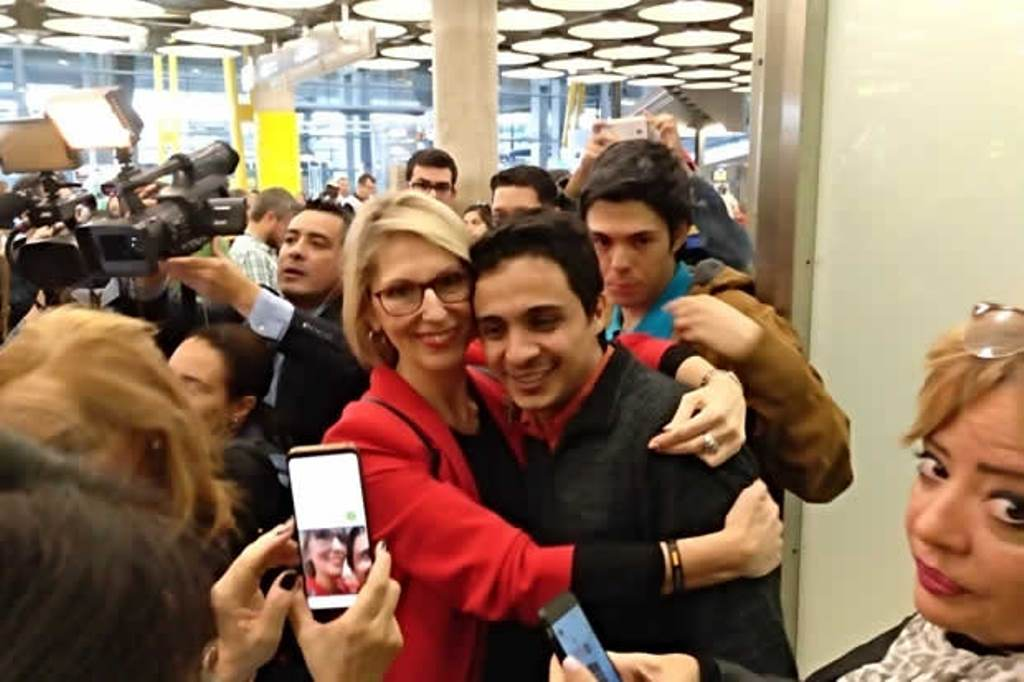
\includegraphics[width=300px]{105.jpg}%
\newline%
%
El joven dirigente político Lorent Saleh, excarcelado el viernes por la autoridades nacionales, enfatizó, a su llegada a España que él no está desterrado: "Estoy en libertad, a mí nadie me va a desterrar de mi país porque pronto volveré", dijo el opositor que en breve iniciará los trámites para lograr el estatus de refugiado.%
\newline%
%
El opositor explicó que "como todo lo que pasa allí" (en el Sebin) fue avisado un día antes de que iba a salir pero sin mayores detalles: "Simplemente me llamaron, me sacaron de la celda y me dijeron que iba a iniciar un nuevo proceso en mi vida pero no sabía qué era; me montaron en un patrulla y me llevaron al aeropuerto", reseñó la agencia Efe.%
\newline%
%
Saleh reconoció este sábado  que, en varias ocasiones pensó en suicidarse porque era "el único mecanismo de defensa" de que disponía para hacer "frente a años de torturas".%
\newline%
%
Saleh llegó al aeropuerto de Madrid acompañado del secretario de Estado español de Cooperación y para Iberoamérica y el Caribe, Juan Pablo de Laiglesia, en un vuelo procedente de Caracas.%
\newline%
%
El funcionario español se había reunido con el canciller Jorge Arreaza, el pasado 10 de octubre en la Casa Amarilla.%
\newline%
%
El gobierno liberó a Saleh luego de 4 años de detención.%
\newline%
%
\end{document}